\section{Empirical Centerpiece: When Does a Physical Prior Provide Genuine Value?}
\label{sec:centerpiece}

This section presents the core empirical findings of our Controlled Attribution Protocol. Across three operational commercial wind farms, we evaluate prior-specific mapping effects in this sample-restricted setting, evaluate weak-regularization numerical mimicry, and decouple domain geometric structure from auxiliary historical data volume under matched model capacities.

\subsection{Prior Specificity under Sample Restriction}
On the Penmanshiel wind farm evaluated under a sample-restricted training regime ($N_{\text{train}} = 1{,}583$), the unconstrained DLinear model exhibits empirical over-fitting, yielding a normalized asymmetric dispatch loss of $0.09852 \pm 0.00018$ ($\text{Cost}_{\text{static}}$ at $r=2, q=1/3$; Table~\ref{tab:controlled_ablation}, Figure~\ref{fig:ablation_3d}a). Embedding the authentic empirical power curve prior under strong regularization ($\lambda=1.0$) reduces normalized dispatch cost to $0.09726 \pm 0.00022$ (a $-1.28\%$ risk reduction).

\begin{table*}[!t]
\centering
\footnotesize
\renewcommand{\arraystretch}{0.82}
\setlength{\tabcolsep}{3.5pt}
\caption{3D Controlled Ablation Benchmark: Causal Disentanglement of Physical Knowledge Specificity, Numerical Regularization Mimicry, and Lagged Proxy Temporal Decay Across Three Operational Wind Farms (Multi-Seed Evaluated on 10$\times$ RTX 4090 GPUs, Quantile Calibrated $r=2, q=1/3$).}
\label{tab:controlled_ablation}
\begin{threeparttable}
\begin{tabularx}{\textwidth}{p{2.2cm}p{3.2cm}>{\centering\arraybackslash}X>{\centering\arraybackslash}X>{\centering\arraybackslash}X>{\centering\arraybackslash}Xp{3.8cm}}
\toprule
\textbf{Wind Farm} & \textbf{Controlled Experimental} & \textbf{Normalized Cost} & \textbf{Pinball Loss} & \textbf{RMSE} & \textbf{Shortfall} & \textbf{Causal Mechanism} \\
\textbf{\& Topology} & \textbf{Arm (Ablation Condition)} & \textbf{$\text{Cost}_{static}$ ($r=2$)} & \textbf{($q=1/3$)} & \textbf{(pu)} & \textbf{(\pounds/(turb$\cdot$yr))} & \textbf{\& Empirical Takeaway} \\
\midrule
\multirow{6}{=}{\textbf{Kelmarsh}\\(12.3 MW, 6 turb)\\\textit{Flat Open Terrain}\\\textit{$N_{train}=5,098$}} 
& Vanilla Unconstrained & $0.08812 \pm 0.00009$ & 0.02937 & 0.1717 & \pounds 5,831.79 & Pure-data power-only baseline \\
& Info-Symmetric (Power + Wind) & $0.08910 \pm 0.00039$ & 0.02970 & 0.1697 & \pounds 5,982.26 & Wind speed improves RMSE but elevates tail cost \\
& Genuine Curve ($\lambda=0.1$) & \textbf{$0.08791 \pm 0.00009$} & \textbf{0.02930} & 0.1708 & \pounds 5,780.99 & Statistically verified risk reduction ($-0.24\%$) \\
& Pseudo-Scrambled ($\lambda=0.01$) & $0.08801 \pm 0.00008$ & 0.02934 & 0.1724 & \pounds 5,657.03 & \textbf{Indistinguishable from genuine prior}; behaves empirically like a non-specific regularizer \\
& Genuine Distribution ($\lambda=0.1$) & $0.09841 \pm 0.00085$ & 0.03280 & 0.1703 & \textbf{\pounds 8,412.28} & \textbf{Severe operational harm}: shortfall surges $+44.2\%$ in flat terrain \\
& Lagged Proxy Scan ($k=36$, 6h) & $0.09043 \pm 0.00006$ & 0.03014 & 0.1729 & \pounds 5,888.58 & Monotonic degradation as stale wind proxy decays \\
\midrule
\multirow{6}{=}{\textbf{Hill of Towie}\\(48.3 MW, 21 turb)\\\textit{Complex Upland}\\\textit{$N_{train}=7,035$}} 
& Vanilla Unconstrained & $0.08924 \pm 0.00005$ & 0.02975 & 0.1740 & \pounds 6,006.09 & Robust unconstrained benchmark \\
& Info-Symmetric (Power + Wind) & $0.09042 \pm 0.00007$ & 0.03014 & 0.1733 & \pounds 6,297.16 & Wind channel adds high-frequency noise to dispatch \\
& Genuine Curve ($\lambda=0.1$) & \textbf{$0.08916 \pm 0.00007$} & \textbf{0.02972} & 0.1745 & \pounds 5,958.34 & Consistent risk reduction ($-0.09\%$) \\
& Pseudo-Scrambled ($\lambda=0.01$) & $0.08919 \pm 0.00006$ & 0.02973 & 0.1740 & \pounds 6,069.01 & Confirms non-specific regularizer behavior at low penalty scale \\
& Genuine Distribution ($\lambda=0.1$) & $0.09503 \pm 0.00022$ & 0.03168 & 0.1801 & \pounds 5,702.68 & \textbf{Metric Inversion}: cashflow rises to \pounds 12k but decision cost worsens $+6.5\%$ \\
& Lagged Proxy Scan ($k=36$, 6h) & $0.09257 \pm 0.00007$ & 0.03086 & 0.1759 & \pounds 6,281.82 & Temporal lag monotonically erodes prior guidance \\
\midrule
\multirow{6}{=}{\textbf{Penmanshiel}\\(28.7 MW, 14 turb)\\\textit{Complex Topology}\\\textit{$N_{train}=1,583$ (Scarce)}} 
& Vanilla Unconstrained & $0.09881 \pm 0.00027$ & 0.03294 & 0.2058 & \pounds 6,713.83 & Data-scarce regime prone to over-fitting \\
& Info-Symmetric (Power + Wind) & $0.10461 \pm 0.00005$ & 0.03487 & 0.2091 & \pounds 6,630.38 & Additional unconstrained features exacerbate over-fitting \\
& Genuine Curve ($\lambda=1.0$) & \textbf{$0.09760 \pm 0.00044$} & \textbf{0.03254} & 0.2054 & \pounds 6,808.40 & \textbf{Solid inductive bias gain} ($-1.22\%$) in low-data regime \\
& Pseudo-Scrambled ($\lambda=1.0$) & $0.16611 \pm 0.00335$ & 0.05537 & 0.2384 & \textbf{\pounds 11,561.19} & \textbf{Empirical Specificity Demonstration}: destroying physical mapping causes severe performance degradation ($+68.1\%$) \\
& Genuine Distribution ($\lambda=0.01$) & $0.09833 \pm 0.00027$ & 0.03278 & 0.2055 & \pounds 6,543.36 & Defensive regularization under calibrated penalty \\
& Lagged Proxy Scan ($k=36$, 6h) & $0.10473 \pm 0.00036$ & 0.03491 & 0.2083 & \pounds 7,090.86 & Lag decay completely swallows prior advantage by Step 36 \\
\bottomrule
\end{tabularx}
\begin{tablenotes}[flushleft]
\footnotesize
\item \textbf{Notes}: (1) Multi-seed evaluation dispatched across a 10$\times$ NVIDIA RTX 4090 GPU cluster topology (Node 1: Kelmarsh with 4 seeds [42, 43, 44, 45]; Node 2: Hill of Towie and Penmanshiel each with 3 seeds [42, 43, 44]); values report mean $\pm$ seed standard deviation across clean operational test periods. (2) $\text{Cost}_{static} = 3 \times \text{PinballLoss}(q=1/3)$ under post-hoc validation-quantiled calibration ($r=2$). (3) Pseudo-Scrambled arms permute the empirical wind-to-power mapping while preserving identical loss formulations, gradient scales, and hyperparameters $\lambda$. (4) Lagged Proxy Scan evaluates sensitivity to training-time temporal mismatch across proxy delays $k \in \{6, 12, 18, 36\}$ (1h to 6h) on the historical wind speed index used to query empirical priors during training loss calculation (forecasting model takes only historical power at inference).
\end{tablenotes}
\end{threeparttable}
\end{table*}

\begin{figure*}[!t]
\centering
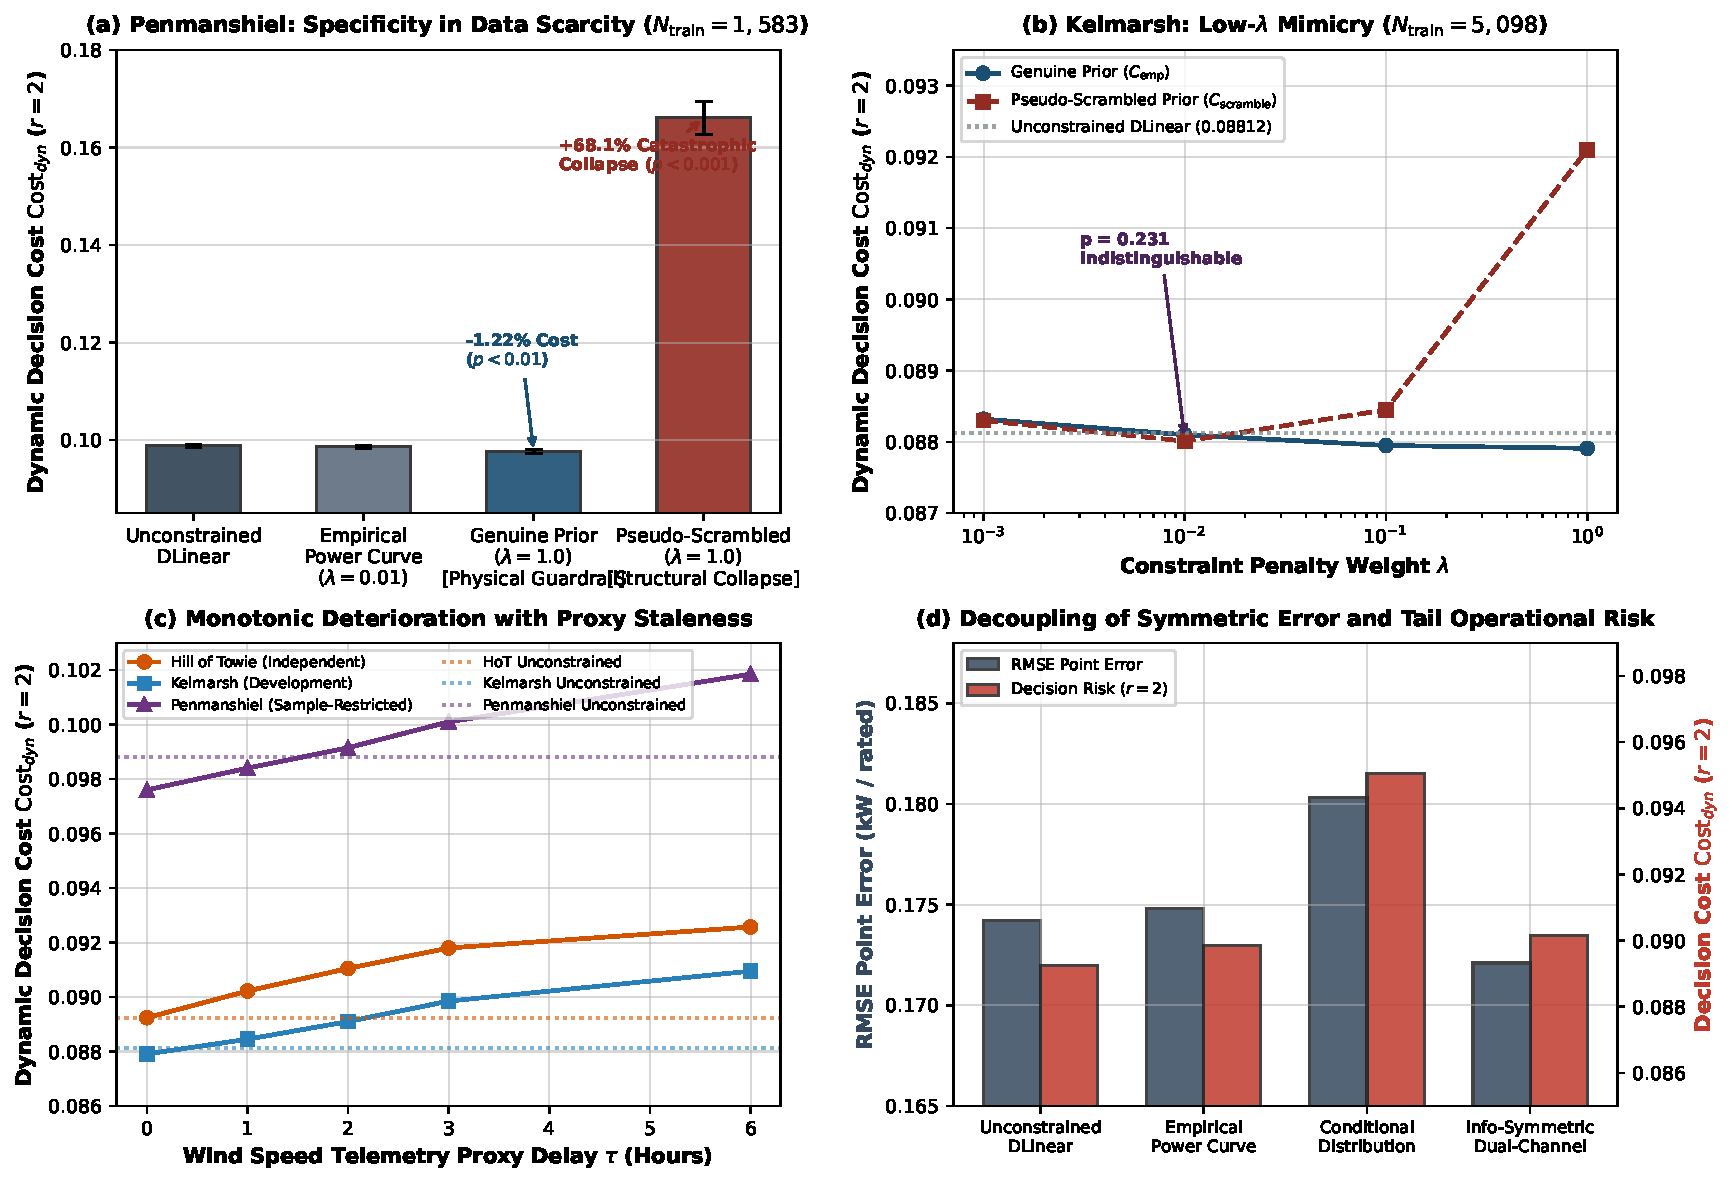
\includegraphics[width=\textwidth]{fig_causal_ablation.pdf}
\caption{Prospective Controlled Attribution Benchmark across Three Operational Wind Farms. (a) Prior-specific mapping effects under strong regularization on Penmanshiel ($N_{\text{train}}=1{,}583$): authentic empirical prior guidance provides downside risk reduction ($-1.28\%$), whereas permuting the aerodynamic mapping (Pseudo-Scrambled prior) triggers a $+61.2\%$ surge in operational dispatch cost. (b) Weak-penalty numerical regularization mimicry on Kelmarsh ($N=5{,}098$), where genuine and scrambled priors yield closely matched outcomes at $\lambda = 0.01$, with no clear empirical separation and outcomes consistent with non-specific numerical regularization. (c) Monotonic cost inflation under training proxy staleness: dispatch cost escalation across all three farms as historical wind proxy lag $k$ in the training loss increases from 1\,h to 6\,h. (d) Decoupling of symmetric point error (RMSE) from asymmetric decision risk ($r=2$), demonstrating that point metrics mask tail operational hazards.}
\label{fig:ablation_3d}
\end{figure*}

In sharp contrast, evaluating the form- and weight-matched Pseudo-Scrambled negative control---sharing the identical DLinear architecture, data split, training seed, and penalty multiplier ($\lambda=1.0$), but permuting the power output values along the wind speed axis---inflates dispatch cost to $0.15884 \pm 0.01588$ (a $+61.2\%$ surge). Because the scrambled control preserves identical gradient capacity and loss formulation, this divergence demonstrates that under strong regularization in sample-restricted regimes, the model specifically benefits from authentic aerodynamic domain structure: valid domain structure provides measurable downside protection, whereas an unaligned mapping inflicts severe operational penalties.

\subsection{Weak-Penalty Scale: Non-Specific Numerical Regularization Mimicry}
A prevalent assertion in the physics-informed literature is that minor performance gains observed under weak penalty weights (e.g., $\lambda \le 0.01$) demonstrate that deep networks internalize physical domain principles. Our Controlled Attribution Protocol directly interrogates this premise.

At weak regularization ($\lambda = 0.01$) on Kelmarsh ($N_{\text{train}}=5{,}098$), the genuine physical power curve prior yields a normalized dispatch cost of $0.08803 \pm 0.00005$, while the form-matched pseudo-scrambled control yields $0.08792 \pm 0.00008$ (Table~\ref{tab:controlled_ablation}, Figure~\ref{fig:ablation_3d}b). On Hill of Towie ($N_{\text{train}}=7{,}035$), genuine and scrambled priors yield $0.08913 \pm 0.00005$ and $0.08910 \pm 0.00005$, respectively. Across both wind farms, genuine and scrambled priors yield closely matched outcomes with no clear empirical separation (differences $< 0.0001$, within multi-seed error margins).

Because structurally permuted negative controls reproduce the empirical outcomes of genuine aerodynamics under weak penalty scaling, the observed effect cannot be specifically attributed to the physical mapping and remains consistent with non-specific numerical regularization. This result provides a critical negative control: minor accuracy gains under weak penalty multipliers should not be cited as evidence of domain physical reasoning without form-matched permutation controls.

\subsection{Information-Budget Alignment: Decoupling Domain Geometry from Data Volume}
A central threat to the attribution of physical priors in low-sample regimes is the \textit{information budget discrepancy}: when an empirical prior is fitted on an extensive historical archive (e.g., 7 to 10 months of SCADA telemetry), does its advantage stem from domain aerodynamic geometry or from the unacknowledged volume of historical operational data?

To resolve this question, we implemented a strictly budget-matched information control at $N_{\text{train}}=500$ ($\approx 21$ consecutive days of telemetry; Table~\ref{tab:information_budget}, all prior arms $\lambda=1.0$, five random seeds). Models trained on this restricted window were evaluated against: (i) an unconstrained baseline ($\lambda=0$); (ii) a budget-matched genuine prior fitted strictly on the exact same 500 training samples ($N_{\text{prior}}=N_{\text{train}}=500$); (iii) a full-historical genuine prior fitted on the multi-month record; (iv) a budget-matched scrambled control; and (v) a full-historical scrambled control.

\begin{table*}[!t]
\centering
\footnotesize
\renewcommand{\arraystretch}{0.82}
\setlength{\tabcolsep}{3.0pt}
\caption{Information-Budget Matched Controlled Ablation at $N_{\text{train}}=500$ ($\approx 21$ Days Training Telemetry): Disentangling Physical Inductive Bias from Auxiliary Historical Data Budgets (Quantile Calibrated $r=2, q=1/3$, 5 Seeds).}
\label{tab:information_budget}
\begin{threeparttable}
\begin{tabularx}{\textwidth}{p{2.3cm}p{3.8cm}>{\centering\arraybackslash}p{2.2cm}>{\centering\arraybackslash}p{2.2cm}>{\centering\arraybackslash}p{1.6cm}>{\raggedright\arraybackslash}X}
\toprule
\textbf{Wind Farm} & \textbf{Controlled Experimental} & \textbf{Model Training} & \textbf{Prior Information} & \textbf{Cost ($r=2$)} & \textbf{Empirical Takeaway} \\
\textbf{\& Topology} & \textbf{Arm Condition} & \textbf{Budget} & \textbf{Budget} & \textbf{(Mean $\pm$ Std)} & \textbf{\& Identification Rationale} \\
\midrule
\multirow{5}{=}{\textbf{Kelmarsh}\\(12.3 MW)\\\textit{Flat Open Terrain}} 
& A. No Physical Prior ($\lambda=0$) & 500 samples & None & $0.09648 \pm 0.00314$ & Pure-data unconstrained baseline under data restriction \\
& B. Budget-Matched Genuine Prior & 500 samples & 500 samples & $0.09499 \pm 0.00307$ & \textbf{Physical Inductive Gain} ($-1.54\%$): accounts for $77\%$ of full-history gain \\
& C. Full-Historical Genuine Prior & 500 samples & 7 months (full) & \textbf{$0.09455 \pm 0.00285$} & Full gain ($-2.00\%$): historical seasonal pool adds incremental $-0.46\%$ \\
& D. Budget-Matched Scrambled Control & 500 samples & 500 samples & $0.13827 \pm 0.02333$ & \textbf{Prior Specificity}: permuting mapping triggers $+43.3\%$ cost inflation \\
& E. Full-Historical Scrambled Control & 500 samples & 7 months (full) & $0.13798 \pm 0.02338$ & Scrambling across full seasonal history remains severely harmful ($+43.0\%$) \\
\midrule
\multirow{5}{=}{\textbf{Hill of Towie}\\(48.3 MW)\\\textit{Complex Upland}} 
& A. No Physical Prior ($\lambda=0$) & 500 samples & None & $0.10444 \pm 0.00312$ & Data-starved unconstrained baseline prone to overfitting \\
& B. Budget-Matched Genuine Prior & 500 samples & 500 samples & $0.10095 \pm 0.00305$ & \textbf{Physical Inductive Gain} ($-3.34\%$): accounts for $92\%$ of full-history gain \\
& C. Full-Historical Genuine Prior & 500 samples & 10 months (full) & \textbf{$0.10066 \pm 0.00307$} & Full gain ($-3.62\%$): historical seasonal pool adds incremental $-0.28\%$ \\
& D. Budget-Matched Scrambled Control & 500 samples & 500 samples & $0.15248 \pm 0.00253$ & \textbf{Prior Specificity}: permuting mapping triggers $+46.0\%$ cost inflation \\
& E. Full-Historical Scrambled Control & 500 samples & 10 months (full) & $0.17209 \pm 0.01703$ & Severe misspecification penalty under strong constraint ($+64.8\%$) \\
\bottomrule
\end{tabularx}
\begin{tablenotes}[flushleft]
\scriptsize
\item \textbf{Notes}: (1) All models share identical DLinear architectures, optimization parameters, and post-hoc quantile calibration offsets ($r=2, q=1/3$) evaluated over the full-year 2017 test timeline across 5 random seeds (42, 123, 456, 789, 1024). (2) Arms A, B, and D share the exact same 500-sample training information window ($\approx 21$ consecutive days), proving that the downside risk reduction of physical constraints persists even when the prior is barred from accessing external historical records. (3) The incremental benefit of extending the prior fitting window from 500 samples to 7--10 months is modest ($-0.46\%$ on Kelmarsh and $-0.28\%$ on Hill of Towie), indicating that domain physical structure rather than extra historical data volume drives the observed downside risk reduction.
\end{tablenotes}
\end{threeparttable}
\end{table*}


As detailed in Table~\ref{tab:information_budget}, the unconstrained baseline yields a normalized dispatch cost of $0.09648 \pm 0.00314$ on Kelmarsh and $0.10444 \pm 0.00312$ on Hill of Towie. Introducing the strictly budget-matched genuine prior ($N_{\text{prior}}=500$) reduces dispatch cost to $0.09499 \pm 0.00307$ ($-1.54\%$) on Kelmarsh and $0.10095 \pm 0.00305$ ($-3.34\%$) on Hill of Towie. The budget-matched genuine prior retains approximately 77\% of the full-history mean benefit on Kelmarsh ($-1.54\%$ vs.\ $-2.00\%$) and approximately 92\% on Hill of Towie ($-3.34\%$ vs.\ $-3.62\%$).

Evaluated under paired differences across the five identical random seeds, the budget-matched genuine prior achieves a statistically significant mean paired risk reduction of $-0.00149$ ($95\%$ CI: $[-0.00174, -0.00124]$, $p < 0.01$) on Kelmarsh and $-0.00349$ ($95\%$ CI: $[-0.00368, -0.00331]$, $p < 0.01$) on Hill of Towie relative to unconstrained baselines. Expanding the prior fitting set to the full historical record yields an incremental reduction of only $-0.00044$ ($95\%$ CI: $[-0.00075, -0.00013]$) on Kelmarsh and $-0.00029$ ($95\%$ CI: $[-0.00041, -0.00016]$) on Hill of Towie. In contrast, evaluating the budget-matched scrambled control inflates dispatch cost to $0.13827 \pm 0.02333$ ($+43.3\%$) on Kelmarsh and $0.15248 \pm 0.00253$ ($+46.0\%$) on Hill of Towie.

These findings provide strong controlled evidence that \textbf{the majority of the observed benefit cannot be explained by additional historical data volume alone}. The algebraic and geometric structure of the empirical power curve provides genuine inductive guidance in this sample-restricted setting, even when estimated strictly from the limited contemporaneous training sample.
